\documentclass[10pt]{beamer}

\usetheme[progressbar=frametitle]{metropolis}
\usepackage{appendixnumberbeamer}





\usepackage{booktabs}
\usepackage[scale=2]{ccicons}

\usepackage{pgfplots}
\usepgfplotslibrary{dateplot}
\usepackage{wrapfig}
\usepackage{xspace}
\newcommand{\themename}{\textbf{\textsc{metropolis}}\xspace}

\title{JEE Linear Algebra using Matrix Computation}
\subtitle{}
\date{}
\author{\quad Harsh Raj\qquad \qquad \qquad \qquad Lakshit Singla \newline MA17BTECH11003 \quad \qquad \qquad EE17BTECH11021}

\begin{document}


\maketitle

\begin{frame}{Problem}
Find the centre of the circle passing through A: \( \left( {\begin{array}{c}
   0 \\
   0 \\
   \end{array} } \right)\) and B: \( \left( {\begin{array}{c}
   1 \\
   0 \\
   \end{array} } \right)\) and touching the circle \(x^2 + y^2 = 9\)\qquad
   (IIT-JEE 2002)
 \begin{figure}[h]
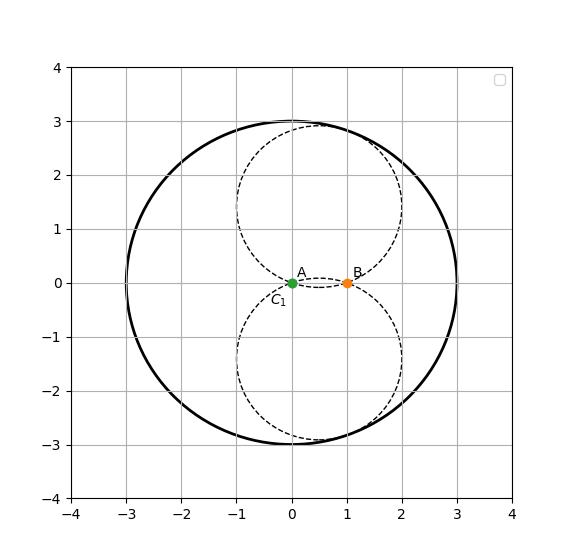
\includegraphics[scale = 0.45]{s1_im1_question.png}

\end{figure}

\end{frame}

\begin{frame}{Given Circle:  \(x^2 + y^2 = 9\)}
  \begin{figure}[h]
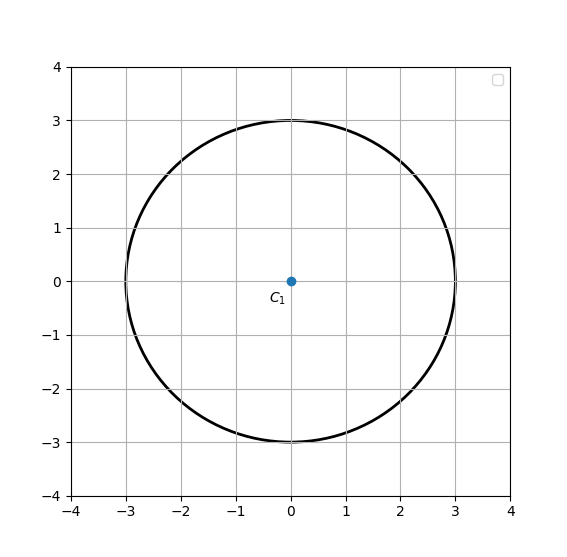
\includegraphics[scale = 0.50]{s2_im1_show_original.png}

\end{figure}   
\end{frame}

\begin{frame}{Scaling}
     \begin{figure}[h]
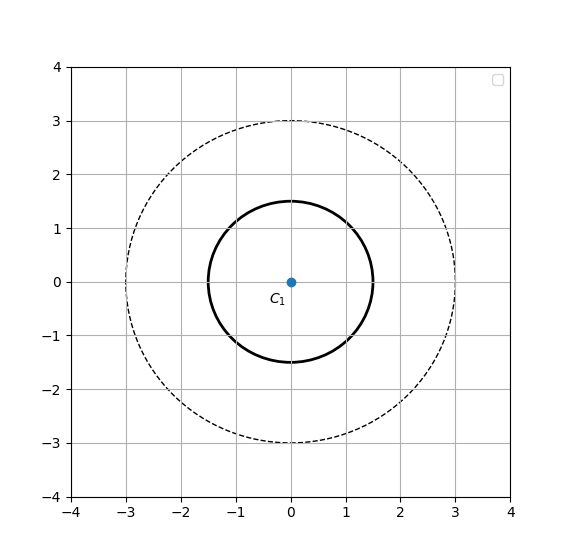
\includegraphics[scale = 0.50]{s2_im3_show_scaling.png}

\end{figure}
\end{frame}

\begin{frame}{Translation}
 \begin{figure}[h]
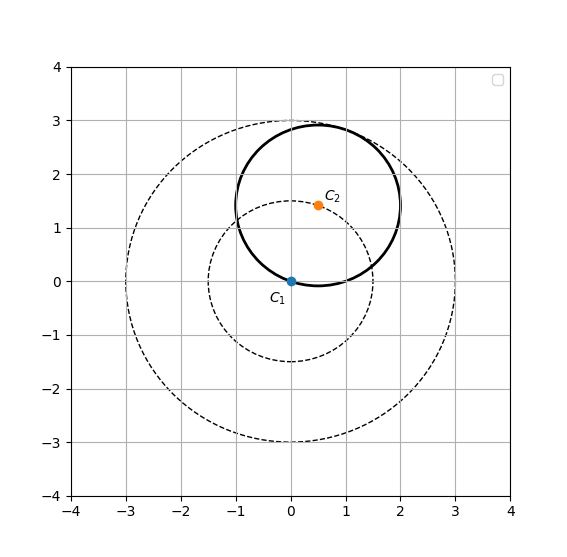
\includegraphics[scale = 0.50]{s2_im3_show_translation.png}

\end{figure}
    
\end{frame}



\begin{frame}{Transformation}
The circle \(G_2\) is obtained from circle \(G_1\) by SCALING and TRANSLATION. The net result in AFFINE Tranformation:
\[T(\textbf{x}) = \alpha\textbf{I}\textbf{x} + (\textbf{C}_2 - \textbf{C}_1)
\]
Where \textbf{I} is Identity matrix

  
\end{frame}

\begin{frame}{Constraints}

\begin{figure}
\centering
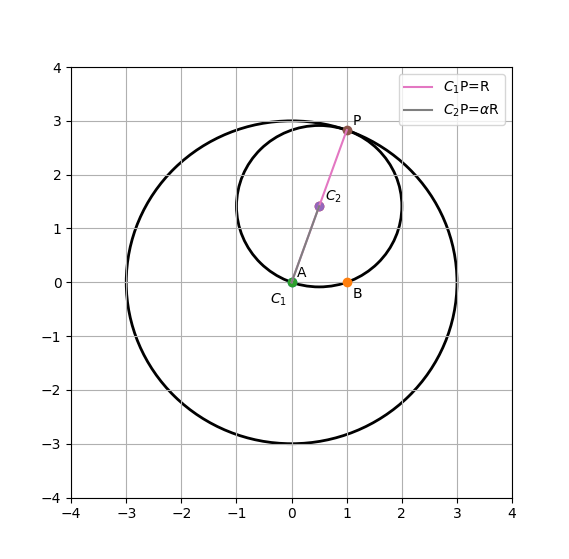
\includegraphics[scale = 0.50]{s3_im1_show_constraints.png}

\end{figure}


    
\end{frame}


\begin{frame}{Contd.}

\(G_1\) has centre \(\textbf{C}_1 = \left( {\begin{array}{c}
   0 \\
   0 \\
   \end{array} } \right)\) and radius \(R = 3\) \newline
   \\

\(G_2\) has centre \(\textbf{C}_2\) and radius \(\alpha R\)\newline \newline
Constraints:\newline \newline
1. \(\|\textbf{C}_2-\textbf{C}_1 \|= R(1-\alpha)\)........as shown in figure \newline \newline
2. Equation of \(G_2\) : \((\textbf{x}-\textbf{C}_2)^{T}(\textbf{x}-\textbf{C}_2) = (\alpha R)^2\)\ \newline \newline is satisfied by \( \left( {\begin{array}{c}
   0 \\
   0 \\
   \end{array} } \right)\) and \( \left( {\begin{array}{c}
   1 \\
   0 \\
   \end{array} } \right)\)
  
\end{frame}

\begin{frame}{Contd.}
\(\textbf{C}_2\textbf{C}_2^{T} = R^2(1-\alpha)^2\)....from Constraint 1 \newline 
\((\textbf{x}-\textbf{C}_2)^{T}(\textbf{x}-\textbf{C}_2) = (\alpha R)^2      \)....from Constraint 2
\[\Rightarrow \textbf{x}^{T}\textbf{x} - \textbf{x}^{T}\textbf{C}_2-\textbf{C}_2^{T}\textbf{x} + \textbf{C}_2^{T}\textbf{C}_2 = (\alpha R)^2
\]
\[\Rightarrow 2\textbf{x}^{T}\textbf{C}_2 = \textbf{x}^{T}\textbf{x} + R^2(1-\alpha^2)-(\alpha R)^2 
\]
\[\Rightarrow 2\textbf{x}^{T}\textbf{C}_2 = \textbf{x}^{T}\textbf{x} + R^2(1-\alpha^2)-(\alpha R)^2 
\]

Above equation is satisfied by  \( \left( {\begin{array}{c}
   0 \\
   0 \\
   \end{array} } \right)\)and \( \left( {\begin{array}{c}
   1 \\
   0 \\
   \end{array} } \right)\) \newline
   Solving gives us: \newline
   \newline
   \(\alpha = 0.5\)\quad;\quad
   \(\textbf{C} _2 =  \left( {\begin{array}{c}
   0.5 \\
   \sqrt{2} \\
   \end{array} } \right)\)\quad OR\quad \(\textbf{C} _2 =  \left( {\begin{array}{c}
   0.5 \\
   -\sqrt{2} \\
   \end{array} } \right)\)
   
 

\end{frame}

\begin{frame}{Final Solution}
 \begin{figure}[h]
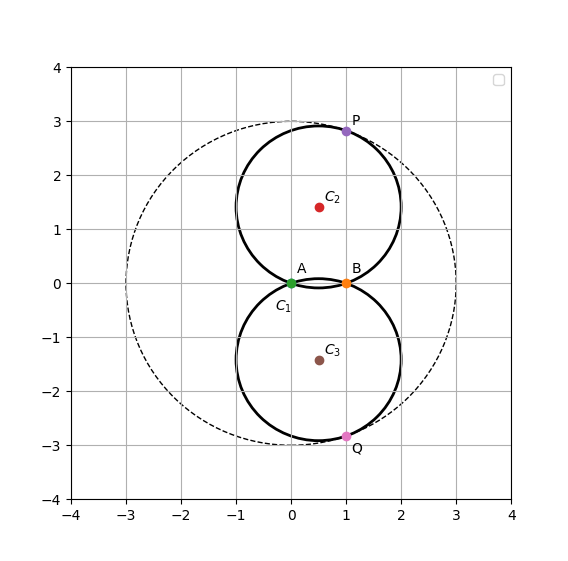
\includegraphics[scale = 0.45]{s5_im1_final_answer.png}

\end{figure}

\quad \quad \qquad  \(\textbf{C}_2 =  \left( {\begin{array}{c}
   0.5 \\
   \sqrt{2} \\
   \end{array} } \right)\)\quad ; \quad\(\textbf{C}_3 =  \left( {\begin{array}{c}
   0.5 \\
   -\sqrt{2} \\
   \end{array} } \right)\)\quad ; \quad \(r = \alpha R = 1.5\)
    
\end{frame}






\end{document}
